% Für Bindekorrektur als optionales Argument "BCORfaktormitmaßeinheit", dann
% sieht auch Option "twoside" vernünftig aus
% Näheres zu "scrartcl" bzw. "scrreprt" und "scrbook" siehe KOMA-Skript Doku
\documentclass[12pt,a4paper,titlepage,headinclude,bibtotoc]{scrartcl}


%---- Allgemeine Layout Einstellungen ------------------------------------------

% Für Kopf und Fußzeilen, siehe auch KOMA-Skript Doku
\usepackage[komastyle]{scrpage2}
\pagestyle{scrheadings}
\setheadsepline{0.5pt}[\color{black}]
\automark[section]{chapter}


%Einstellungen für Figuren- und Tabellenbeschriftungen
\setkomafont{captionlabel}{\sffamily\bfseries}
\setcapindent{0em}


%---- Weitere Pakete -----------------------------------------------------------
% Die Pakete sind alle in der TeX Live Distribution enthalten. Wichtige Adressen
% www.ctan.org, www.dante.de

% Sprachunterstützung
\usepackage[ngerman]{babel}

% Benutzung von Umlauten direkt im Text
% entweder "latin1" oder "utf8"
\usepackage[utf8]{inputenc}

% Pakete mit Mathesymbolen und zur Beseitigung von Schwächen der Mathe-Umgebung
\usepackage{latexsym,exscale,stmaryrd,amssymb,amsmath}

% Weitere Symbole
\usepackage[nointegrals]{wasysym}
\usepackage{eurosym}

% Anderes Literaturverzeichnisformat
%\usepackage[square,sort&compress]{natbib}

% Für Farbe
\usepackage{color}

% Zur Graphikausgabe
%Beipiel: \includegraphics[width=\textwidth]{grafik.png}
\usepackage{graphicx}

% Text umfließt Graphiken und Tabellen
% Beispiel:
% \begin{wrapfigure}[Zeilenanzahl]{"l" oder "r"}{breite}
%   \centering
%   \includegraphics[width=...]{grafik}
%   \caption{Beschriftung} 
%   \label{fig:grafik}
% \end{wrapfigure}
\usepackage{wrapfig}

% Mehrere Abbildungen nebeneinander
% Beispiel:
% \begin{figure}[htb]
%   \centering
%   \subfigure[Beschriftung 1\label{fig:label1}]
%   {\includegraphics[width=0.49\textwidth]{grafik1}}
%   \hfill
%   \subfigure[Beschriftung 2\label{fig:label2}]
%   {\includegraphics[width=0.49\textwidth]{grafik2}}
%   \caption{Beschriftung allgemein}
%   \label{fig:label-gesamt}
% \end{figure}
\usepackage{subfigure}

% Caption neben Abbildung
% Beispiel:
% \sidecaptionvpos{figure}{"c" oder "t" oder "b"}
% \begin{SCfigure}[rel. Breite (normalerweise = 1)][hbt]
%   \centering
%   \includegraphics[width=0.5\textwidth]{grafik.png}
%   \caption{Beschreibung}
%   \label{fig:}
% \end{SCfigure}
\usepackage{sidecap}

% Befehl für "Entspricht"-Zeichen
\newcommand{\corresponds}{\ensuremath{\mathrel{\widehat{=}}}}
% Befehl für Errorfunction
\newcommand{\erf}[1]{\text{ erf}\ensuremath{\left( #1 \right)}}

%Fußnoten zwingend auf diese Seite setzen
\interfootnotelinepenalty=1000

%Für chemische Formeln (von www.dante.de)
%% Anpassung an LaTeX(2e) von Bernd Raichle
\makeatletter
\DeclareRobustCommand{\chemical}[1]{%
  {\(\m@th
   \edef\resetfontdimens{\noexpand\)%
       \fontdimen16\textfont2=\the\fontdimen16\textfont2
       \fontdimen17\textfont2=\the\fontdimen17\textfont2\relax}%
   \fontdimen16\textfont2=2.7pt \fontdimen17\textfont2=2.7pt
   \mathrm{#1}%
   \resetfontdimens}}
\makeatother

%Honecker-Kasten mit $$\shadowbox{$xxxx$}$$
\usepackage{fancybox}

%SI-Package
\usepackage{siunitx}

%keine Einrückung, wenn Latex doppelte Leerzeile
\parindent0pt

%Bibliography \bibliography{literatur} und \cite{gerthsen}
%\usepackage{cite}
\usepackage{babelbib}
\selectbiblanguage{ngerman}

\begin{document}

\begin{titlepage}
\centering
\textsc{\Large Anfängerpraktikum der Fakultät für
  Physik,\\[1.5ex] Universität Göttingen}

\vspace*{3.5cm}

\rule{\textwidth}{1pt}\\[0.5cm]
{\huge \bfseries
  Magnetfelder von Spulen\\[1.5ex]
  Protokoll}\\[0.5cm]
\rule{\textwidth}{1pt}

\vspace*{3.5cm}

\begin{Large}
\begin{tabular}{ll}
Praktikant: &  Michael Lohmann\\
 &  Felix Kurtz\\
% &  Kevin Lüdemann\\
% &  Skrollan Detzler\\
 E-Mail: & m.lohmann@stud.uni-goettingen.de\\
 &  felix.kurtz@stud.uni-goettingen.de\\
% &  kevin.luedemann@stud.uni-goettingen.de\\
% &  skrollan.detzler@stud.uni-goettingen.de\\
 Betreuer: & Björn Klaas\\
 Versuchsdatum: & 05.09.2014\\
\end{tabular}
\end{Large}

\vspace*{0.8cm}

\begin{Large}
\fbox{
  \begin{minipage}[t][2.5cm][t]{6cm} 
    Testat:
  \end{minipage}
}
\end{Large}

\end{titlepage}

\tableofcontents

\newpage

\section{Einleitung}
\label{sec:einleitung}
Spulen sind für die Transformation von Spannungen essentiell.
Jede Spule besitzt ein charakteristisches Magnetfeld mit dessen genauer Kenntnis man zum Beispiel Untersuchungen wie Magnetresonanztomographie ermöglichen kann.
Dafür ist allerdings eine sehr genaue Beschreibung des Magnetfeldes der Spule notwendig.
Für zwei Spulen wurde es hier durchgeführt.

\section{Theorie}
\label{sec:theorie}
\cite{gerthsen}


\section{Durchführung}
\label{sec:durchfuehrung}
Zuerst muss der Stromintegrator kalibriert werden.
Dazu \\
\begin{figure}[!htb]
	 \centering
	 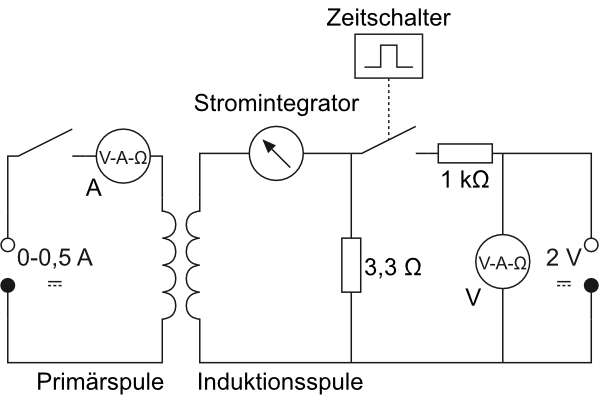
\includegraphics[scale=1.0]{IndSpuleAufbau.png}
	\caption{Magnetfeldmessung mit der Induktionsspule \cite[Datum: 09.10.2014]{LP13}}	 
	 \label{fig:IndSpule}
\end{figure}
Danach misst man das Magnetfeld der Langen Spule (Primärspule) mit der Induktionsspule nach dem Aufbau aus Abb. \ref{fig:IndSpule}, indem der Schalter im Primärkreis kurz geöffnet und wieder geschlossen wird.
Der durch den erzeugten Spannungspuls resultierende Strom wird über das Ladungsmessgerät integriert.
Für verschiedene Positionen auf der Spulenachse wird die Anzeige des Ladungsmessgerätes notiert.
Die Schrittweite beträgt dabei $2\,$cm und die Messung wird auch außerhalb der Spule fortgeführt.\\
Zu den weiteren Messungen wird die Hall-Sonde benutzt.
Diese schließt man an den Strom an und auf dem Display erscheint das gemessene Magnetfeld in Gauss.
Man startet bei allen drei Spulen (inkl. Helmholtzspule) in der Mitte der Spule und bewegt die Sonde bei jeder Messung um $1\,$cm heraus.
Zuletzt werden die Daten der einzelnen Spulen wie Länge, Durchmesser und Wicklungszahl notiert.


\section{Auswertung}
\label{sec:auswertung}
\subsection{Eichen des Ladungsmessgeräts}
\begin{align}
		R_\text{ges}=R_1+\left(\frac{1}{R_2}+\frac{1}{R_L+R_\text{int}}\right)^{-1}
\end{align}

\begin{align*}
	R_2 I_2=(R_L+R_\text{int})I_\kappa
\end{align*}

\begin{align*}
	I_\text{ges}=I_\kappa+I_2=I_\kappa\left(1+\frac{R_L+R_\text{int}}{R_2}\right)
\end{align*}

\begin{align}
	R_\kappa=\frac{U}{I_\kappa}=\frac{U}{I_\text{ges}}\left(1+\frac{R_L+R_\text{int}}{R_2}\right)=R_\text{ges}\left(1+\frac{R_L+R_\text{int}}{R_2}\right)
\end{align}

\begin{figure}[!htb]
	\centering
	% GNUPLOT: LaTeX picture with Postscript
\begingroup
  \makeatletter
  \providecommand\color[2][]{%
    \GenericError{(gnuplot) \space\space\space\@spaces}{%
      Package color not loaded in conjunction with
      terminal option `colourtext'%
    }{See the gnuplot documentation for explanation.%
    }{Either use 'blacktext' in gnuplot or load the package
      color.sty in LaTeX.}%
    \renewcommand\color[2][]{}%
  }%
  \providecommand\includegraphics[2][]{%
    \GenericError{(gnuplot) \space\space\space\@spaces}{%
      Package graphicx or graphics not loaded%
    }{See the gnuplot documentation for explanation.%
    }{The gnuplot epslatex terminal needs graphicx.sty or graphics.sty.}%
    \renewcommand\includegraphics[2][]{}%
  }%
  \providecommand\rotatebox[2]{#2}%
  \@ifundefined{ifGPcolor}{%
    \newif\ifGPcolor
    \GPcolortrue
  }{}%
  \@ifundefined{ifGPblacktext}{%
    \newif\ifGPblacktext
    \GPblacktexttrue
  }{}%
  % define a \g@addto@macro without @ in the name:
  \let\gplgaddtomacro\g@addto@macro
  % define empty templates for all commands taking text:
  \gdef\gplbacktext{}%
  \gdef\gplfronttext{}%
  \makeatother
  \ifGPblacktext
    % no textcolor at all
    \def\colorrgb#1{}%
    \def\colorgray#1{}%
  \else
    % gray or color?
    \ifGPcolor
      \def\colorrgb#1{\color[rgb]{#1}}%
      \def\colorgray#1{\color[gray]{#1}}%
      \expandafter\def\csname LTw\endcsname{\color{white}}%
      \expandafter\def\csname LTb\endcsname{\color{black}}%
      \expandafter\def\csname LTa\endcsname{\color{black}}%
      \expandafter\def\csname LT0\endcsname{\color[rgb]{1,0,0}}%
      \expandafter\def\csname LT1\endcsname{\color[rgb]{0,1,0}}%
      \expandafter\def\csname LT2\endcsname{\color[rgb]{0,0,1}}%
      \expandafter\def\csname LT3\endcsname{\color[rgb]{1,0,1}}%
      \expandafter\def\csname LT4\endcsname{\color[rgb]{0,1,1}}%
      \expandafter\def\csname LT5\endcsname{\color[rgb]{1,1,0}}%
      \expandafter\def\csname LT6\endcsname{\color[rgb]{0,0,0}}%
      \expandafter\def\csname LT7\endcsname{\color[rgb]{1,0.3,0}}%
      \expandafter\def\csname LT8\endcsname{\color[rgb]{0.5,0.5,0.5}}%
    \else
      % gray
      \def\colorrgb#1{\color{black}}%
      \def\colorgray#1{\color[gray]{#1}}%
      \expandafter\def\csname LTw\endcsname{\color{white}}%
      \expandafter\def\csname LTb\endcsname{\color{black}}%
      \expandafter\def\csname LTa\endcsname{\color{black}}%
      \expandafter\def\csname LT0\endcsname{\color{black}}%
      \expandafter\def\csname LT1\endcsname{\color{black}}%
      \expandafter\def\csname LT2\endcsname{\color{black}}%
      \expandafter\def\csname LT3\endcsname{\color{black}}%
      \expandafter\def\csname LT4\endcsname{\color{black}}%
      \expandafter\def\csname LT5\endcsname{\color{black}}%
      \expandafter\def\csname LT6\endcsname{\color{black}}%
      \expandafter\def\csname LT7\endcsname{\color{black}}%
      \expandafter\def\csname LT8\endcsname{\color{black}}%
    \fi
  \fi
  \setlength{\unitlength}{0.0500bp}%
  \begin{picture}(7200.00,5040.00)%
    \gplgaddtomacro\gplbacktext{%
      \csname LTb\endcsname%
      \put(1254,704){\makebox(0,0)[r]{\strut{} 0}}%
      \put(1254,1074){\makebox(0,0)[r]{\strut{} 0.1}}%
      \put(1254,1444){\makebox(0,0)[r]{\strut{} 0.2}}%
      \put(1254,1815){\makebox(0,0)[r]{\strut{} 0.3}}%
      \put(1254,2185){\makebox(0,0)[r]{\strut{} 0.4}}%
      \put(1254,2555){\makebox(0,0)[r]{\strut{} 0.5}}%
      \put(1254,2925){\makebox(0,0)[r]{\strut{} 0.6}}%
      \put(1254,3295){\makebox(0,0)[r]{\strut{} 0.7}}%
      \put(1254,3665){\makebox(0,0)[r]{\strut{} 0.8}}%
      \put(1254,4036){\makebox(0,0)[r]{\strut{} 0.9}}%
      \put(1254,4406){\makebox(0,0)[r]{\strut{} 1}}%
      \put(1254,4776){\makebox(0,0)[r]{\strut{} 1.1}}%
      \put(1386,484){\makebox(0,0){\strut{} 0}}%
      \put(2005,484){\makebox(0,0){\strut{} 100}}%
      \put(2624,484){\makebox(0,0){\strut{} 200}}%
      \put(3243,484){\makebox(0,0){\strut{} 300}}%
      \put(3862,484){\makebox(0,0){\strut{} 400}}%
      \put(4482,484){\makebox(0,0){\strut{} 500}}%
      \put(5101,484){\makebox(0,0){\strut{} 600}}%
      \put(5720,484){\makebox(0,0){\strut{} 700}}%
      \put(6339,484){\makebox(0,0){\strut{} 800}}%
      \put(6958,484){\makebox(0,0){\strut{} 900}}%
      \put(484,2740){\rotatebox{90}{\makebox(0,0){\strut{}Ladung [mC]}}}%
      \put(4172,154){\makebox(0,0){\strut{}Skalen-Teile}}%
    }%
    \gplgaddtomacro\gplfronttext{%
      \csname LTb\endcsname%
      \put(3762,4603){\makebox(0,0)[r]{\strut{}Messwerte}}%
      \csname LTb\endcsname%
      \put(3762,4383){\makebox(0,0)[r]{\strut{}Regressionsgerade}}%
    }%
    \gplbacktext
    \put(0,0){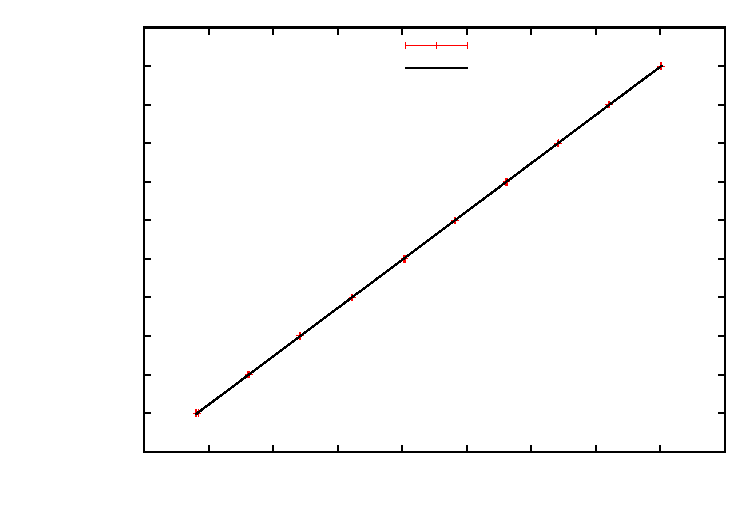
\includegraphics{Eichen}}%
    \gplfronttext
  \end{picture}%
\endgroup

	\caption{Ladung in Abhängigkeit der angezeigten Skalenteile.}
	\label{fig:Eichen}
\end{figure}

\begin{align}
	\kappa=(426.9 \pm 0.4)\,\si{\pico\coulomb\per Skt.}
\end{align}
Da der Fehler so gering ist wird er in der folgenden Berechnung nicht berücksichtigt.
\subsection{Vergleich der beiden Messmethoden}
\begin{figure}[!htb]
	\centering
	% GNUPLOT: LaTeX picture with Postscript
\begingroup
  \makeatletter
  \providecommand\color[2][]{%
    \GenericError{(gnuplot) \space\space\space\@spaces}{%
      Package color not loaded in conjunction with
      terminal option `colourtext'%
    }{See the gnuplot documentation for explanation.%
    }{Either use 'blacktext' in gnuplot or load the package
      color.sty in LaTeX.}%
    \renewcommand\color[2][]{}%
  }%
  \providecommand\includegraphics[2][]{%
    \GenericError{(gnuplot) \space\space\space\@spaces}{%
      Package graphicx or graphics not loaded%
    }{See the gnuplot documentation for explanation.%
    }{The gnuplot epslatex terminal needs graphicx.sty or graphics.sty.}%
    \renewcommand\includegraphics[2][]{}%
  }%
  \providecommand\rotatebox[2]{#2}%
  \@ifundefined{ifGPcolor}{%
    \newif\ifGPcolor
    \GPcolortrue
  }{}%
  \@ifundefined{ifGPblacktext}{%
    \newif\ifGPblacktext
    \GPblacktexttrue
  }{}%
  % define a \g@addto@macro without @ in the name:
  \let\gplgaddtomacro\g@addto@macro
  % define empty templates for all commands taking text:
  \gdef\gplbacktext{}%
  \gdef\gplfronttext{}%
  \makeatother
  \ifGPblacktext
    % no textcolor at all
    \def\colorrgb#1{}%
    \def\colorgray#1{}%
  \else
    % gray or color?
    \ifGPcolor
      \def\colorrgb#1{\color[rgb]{#1}}%
      \def\colorgray#1{\color[gray]{#1}}%
      \expandafter\def\csname LTw\endcsname{\color{white}}%
      \expandafter\def\csname LTb\endcsname{\color{black}}%
      \expandafter\def\csname LTa\endcsname{\color{black}}%
      \expandafter\def\csname LT0\endcsname{\color[rgb]{1,0,0}}%
      \expandafter\def\csname LT1\endcsname{\color[rgb]{0,1,0}}%
      \expandafter\def\csname LT2\endcsname{\color[rgb]{0,0,1}}%
      \expandafter\def\csname LT3\endcsname{\color[rgb]{1,0,1}}%
      \expandafter\def\csname LT4\endcsname{\color[rgb]{0,1,1}}%
      \expandafter\def\csname LT5\endcsname{\color[rgb]{1,1,0}}%
      \expandafter\def\csname LT6\endcsname{\color[rgb]{0,0,0}}%
      \expandafter\def\csname LT7\endcsname{\color[rgb]{1,0.3,0}}%
      \expandafter\def\csname LT8\endcsname{\color[rgb]{0.5,0.5,0.5}}%
    \else
      % gray
      \def\colorrgb#1{\color{black}}%
      \def\colorgray#1{\color[gray]{#1}}%
      \expandafter\def\csname LTw\endcsname{\color{white}}%
      \expandafter\def\csname LTb\endcsname{\color{black}}%
      \expandafter\def\csname LTa\endcsname{\color{black}}%
      \expandafter\def\csname LT0\endcsname{\color{black}}%
      \expandafter\def\csname LT1\endcsname{\color{black}}%
      \expandafter\def\csname LT2\endcsname{\color{black}}%
      \expandafter\def\csname LT3\endcsname{\color{black}}%
      \expandafter\def\csname LT4\endcsname{\color{black}}%
      \expandafter\def\csname LT5\endcsname{\color{black}}%
      \expandafter\def\csname LT6\endcsname{\color{black}}%
      \expandafter\def\csname LT7\endcsname{\color{black}}%
      \expandafter\def\csname LT8\endcsname{\color{black}}%
    \fi
  \fi
  \setlength{\unitlength}{0.0500bp}%
  \begin{picture}(7200.00,5040.00)%
    \gplgaddtomacro\gplbacktext{%
      \csname LTb\endcsname%
      \put(814,1804){\makebox(0,0)[r]{\strut{} 0}}%
      \put(814,2228){\makebox(0,0)[r]{\strut{} 2}}%
      \put(814,2653){\makebox(0,0)[r]{\strut{} 4}}%
      \put(814,3077){\makebox(0,0)[r]{\strut{} 6}}%
      \put(814,3502){\makebox(0,0)[r]{\strut{} 8}}%
      \put(814,3926){\makebox(0,0)[r]{\strut{} 10}}%
      \put(814,4351){\makebox(0,0)[r]{\strut{} 12}}%
      \put(814,4775){\makebox(0,0)[r]{\strut{} 14}}%
      \put(946,1584){\makebox(0,0){\strut{}-20}}%
      \put(1783,1584){\makebox(0,0){\strut{}-10}}%
      \put(2619,1584){\makebox(0,0){\strut{} 0}}%
      \put(3456,1584){\makebox(0,0){\strut{} 10}}%
      \put(4293,1584){\makebox(0,0){\strut{} 20}}%
      \put(5130,1584){\makebox(0,0){\strut{} 30}}%
      \put(5966,1584){\makebox(0,0){\strut{} 40}}%
      \put(6803,1584){\makebox(0,0){\strut{} 50}}%
      \put(176,3289){\rotatebox{-270}{\makebox(0,0){\strut{}Magnetfeld [Gs]}}}%
      \put(3874,1254){\makebox(0,0){\strut{}Position [cm]}}%
    }%
    \gplgaddtomacro\gplfronttext{%
      \csname LTb\endcsname%
      \put(4833,833){\makebox(0,0)[r]{\strut{}Induktion}}%
      \csname LTb\endcsname%
      \put(4833,613){\makebox(0,0)[r]{\strut{}Hallsonde}}%
      \csname LTb\endcsname%
      \put(4833,393){\makebox(0,0)[r]{\strut{}Näherung lange Spule}}%
      \csname LTb\endcsname%
      \put(4833,173){\makebox(0,0)[r]{\strut{}theoretischer Verlauf}}%
    }%
    \gplbacktext
    \put(0,0){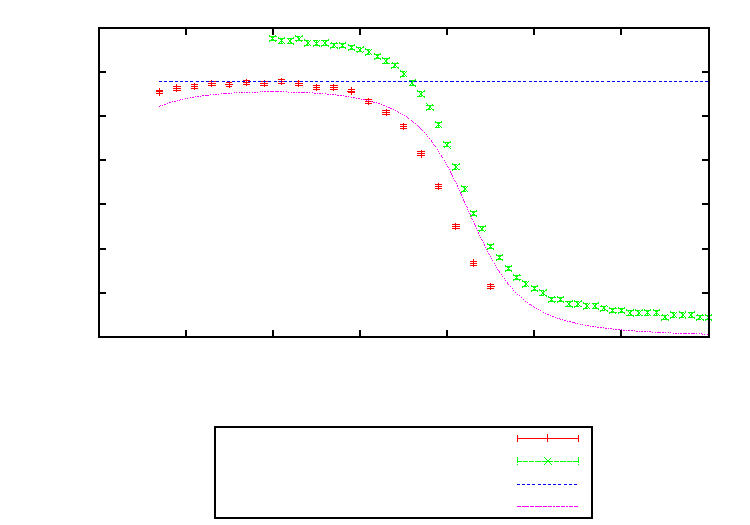
\includegraphics{LangIndHall}}%
    \gplfronttext
  \end{picture}%
\endgroup

	\caption{Verlauf des Magnetfeldes: Vergleich der beiden Messmethoden mit der Theorie anhand der Langen Spule.}
	\label{fig:LangIndHall}
\end{figure}
\subsection{Messung mit der Hallsonde}
\begin{figure}[!htb]
	\centering
	% GNUPLOT: LaTeX picture with Postscript
\begingroup
  \makeatletter
  \providecommand\color[2][]{%
    \GenericError{(gnuplot) \space\space\space\@spaces}{%
      Package color not loaded in conjunction with
      terminal option `colourtext'%
    }{See the gnuplot documentation for explanation.%
    }{Either use 'blacktext' in gnuplot or load the package
      color.sty in LaTeX.}%
    \renewcommand\color[2][]{}%
  }%
  \providecommand\includegraphics[2][]{%
    \GenericError{(gnuplot) \space\space\space\@spaces}{%
      Package graphicx or graphics not loaded%
    }{See the gnuplot documentation for explanation.%
    }{The gnuplot epslatex terminal needs graphicx.sty or graphics.sty.}%
    \renewcommand\includegraphics[2][]{}%
  }%
  \providecommand\rotatebox[2]{#2}%
  \@ifundefined{ifGPcolor}{%
    \newif\ifGPcolor
    \GPcolortrue
  }{}%
  \@ifundefined{ifGPblacktext}{%
    \newif\ifGPblacktext
    \GPblacktexttrue
  }{}%
  % define a \g@addto@macro without @ in the name:
  \let\gplgaddtomacro\g@addto@macro
  % define empty templates for all commands taking text:
  \gdef\gplbacktext{}%
  \gdef\gplfronttext{}%
  \makeatother
  \ifGPblacktext
    % no textcolor at all
    \def\colorrgb#1{}%
    \def\colorgray#1{}%
  \else
    % gray or color?
    \ifGPcolor
      \def\colorrgb#1{\color[rgb]{#1}}%
      \def\colorgray#1{\color[gray]{#1}}%
      \expandafter\def\csname LTw\endcsname{\color{white}}%
      \expandafter\def\csname LTb\endcsname{\color{black}}%
      \expandafter\def\csname LTa\endcsname{\color{black}}%
      \expandafter\def\csname LT0\endcsname{\color[rgb]{1,0,0}}%
      \expandafter\def\csname LT1\endcsname{\color[rgb]{0,1,0}}%
      \expandafter\def\csname LT2\endcsname{\color[rgb]{0,0,1}}%
      \expandafter\def\csname LT3\endcsname{\color[rgb]{1,0,1}}%
      \expandafter\def\csname LT4\endcsname{\color[rgb]{0,1,1}}%
      \expandafter\def\csname LT5\endcsname{\color[rgb]{1,1,0}}%
      \expandafter\def\csname LT6\endcsname{\color[rgb]{0,0,0}}%
      \expandafter\def\csname LT7\endcsname{\color[rgb]{1,0.3,0}}%
      \expandafter\def\csname LT8\endcsname{\color[rgb]{0.5,0.5,0.5}}%
    \else
      % gray
      \def\colorrgb#1{\color{black}}%
      \def\colorgray#1{\color[gray]{#1}}%
      \expandafter\def\csname LTw\endcsname{\color{white}}%
      \expandafter\def\csname LTb\endcsname{\color{black}}%
      \expandafter\def\csname LTa\endcsname{\color{black}}%
      \expandafter\def\csname LT0\endcsname{\color{black}}%
      \expandafter\def\csname LT1\endcsname{\color{black}}%
      \expandafter\def\csname LT2\endcsname{\color{black}}%
      \expandafter\def\csname LT3\endcsname{\color{black}}%
      \expandafter\def\csname LT4\endcsname{\color{black}}%
      \expandafter\def\csname LT5\endcsname{\color{black}}%
      \expandafter\def\csname LT6\endcsname{\color{black}}%
      \expandafter\def\csname LT7\endcsname{\color{black}}%
      \expandafter\def\csname LT8\endcsname{\color{black}}%
    \fi
  \fi
  \setlength{\unitlength}{0.0500bp}%
  \begin{picture}(7200.00,5040.00)%
    \gplgaddtomacro\gplbacktext{%
      \csname LTb\endcsname%
      \put(814,2244){\makebox(0,0)[r]{\strut{}-2}}%
      \put(814,2560){\makebox(0,0)[r]{\strut{} 0}}%
      \put(814,2877){\makebox(0,0)[r]{\strut{} 2}}%
      \put(814,3193){\makebox(0,0)[r]{\strut{} 4}}%
      \put(814,3510){\makebox(0,0)[r]{\strut{} 6}}%
      \put(814,3826){\makebox(0,0)[r]{\strut{} 8}}%
      \put(814,4142){\makebox(0,0)[r]{\strut{} 10}}%
      \put(814,4459){\makebox(0,0)[r]{\strut{} 12}}%
      \put(814,4775){\makebox(0,0)[r]{\strut{} 14}}%
      \put(946,2024){\makebox(0,0){\strut{} 0}}%
      \put(2117,2024){\makebox(0,0){\strut{} 10}}%
      \put(3289,2024){\makebox(0,0){\strut{} 20}}%
      \put(4460,2024){\makebox(0,0){\strut{} 30}}%
      \put(5632,2024){\makebox(0,0){\strut{} 40}}%
      \put(6803,2024){\makebox(0,0){\strut{} 50}}%
      \put(176,3509){\rotatebox{-270}{\makebox(0,0){\strut{}Magnetfeld [Gs]}}}%
      \put(3874,1694){\makebox(0,0){\strut{}Position [cm]}}%
    }%
    \gplgaddtomacro\gplfronttext{%
      \csname LTb\endcsname%
      \put(5691,1273){\makebox(0,0)[r]{\strut{}Lange Spule}}%
      \csname LTb\endcsname%
      \put(5691,1053){\makebox(0,0)[r]{\strut{}Lange Spule: Näherung lange Spule}}%
      \csname LTb\endcsname%
      \put(5691,833){\makebox(0,0)[r]{\strut{}Lange Spule: theoretischer Verlauf}}%
      \csname LTb\endcsname%
      \put(5691,613){\makebox(0,0)[r]{\strut{}Dicke Spule}}%
      \csname LTb\endcsname%
      \put(5691,393){\makebox(0,0)[r]{\strut{}Dicke Spule: Näherung lange Spule}}%
      \csname LTb\endcsname%
      \put(5691,173){\makebox(0,0)[r]{\strut{}Dicke Spule: theoretischer Verlauf}}%
    }%
    \gplbacktext
    \put(0,0){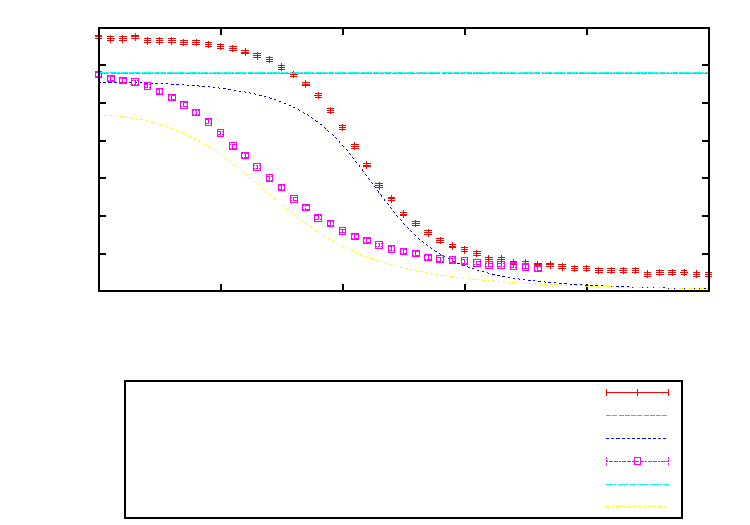
\includegraphics{Hall}}%
    \gplfronttext
  \end{picture}%
\endgroup

	\caption{Verlauf des Magnetfeldes: Vergleich der langen und der dicken Spule sowie jeweils mit der Theorie.}
	\label{fig:HallVergleich}
\end{figure}
\subsection{Homogenität der Magnetfelder}
\begin{figure}[!htb]
	\centering
	% GNUPLOT: LaTeX picture with Postscript
\begingroup
  \makeatletter
  \providecommand\color[2][]{%
    \GenericError{(gnuplot) \space\space\space\@spaces}{%
      Package color not loaded in conjunction with
      terminal option `colourtext'%
    }{See the gnuplot documentation for explanation.%
    }{Either use 'blacktext' in gnuplot or load the package
      color.sty in LaTeX.}%
    \renewcommand\color[2][]{}%
  }%
  \providecommand\includegraphics[2][]{%
    \GenericError{(gnuplot) \space\space\space\@spaces}{%
      Package graphicx or graphics not loaded%
    }{See the gnuplot documentation for explanation.%
    }{The gnuplot epslatex terminal needs graphicx.sty or graphics.sty.}%
    \renewcommand\includegraphics[2][]{}%
  }%
  \providecommand\rotatebox[2]{#2}%
  \@ifundefined{ifGPcolor}{%
    \newif\ifGPcolor
    \GPcolortrue
  }{}%
  \@ifundefined{ifGPblacktext}{%
    \newif\ifGPblacktext
    \GPblacktexttrue
  }{}%
  % define a \g@addto@macro without @ in the name:
  \let\gplgaddtomacro\g@addto@macro
  % define empty templates for all commands taking text:
  \gdef\gplbacktext{}%
  \gdef\gplfronttext{}%
  \makeatother
  \ifGPblacktext
    % no textcolor at all
    \def\colorrgb#1{}%
    \def\colorgray#1{}%
  \else
    % gray or color?
    \ifGPcolor
      \def\colorrgb#1{\color[rgb]{#1}}%
      \def\colorgray#1{\color[gray]{#1}}%
      \expandafter\def\csname LTw\endcsname{\color{white}}%
      \expandafter\def\csname LTb\endcsname{\color{black}}%
      \expandafter\def\csname LTa\endcsname{\color{black}}%
      \expandafter\def\csname LT0\endcsname{\color[rgb]{1,0,0}}%
      \expandafter\def\csname LT1\endcsname{\color[rgb]{0,1,0}}%
      \expandafter\def\csname LT2\endcsname{\color[rgb]{0,0,1}}%
      \expandafter\def\csname LT3\endcsname{\color[rgb]{1,0,1}}%
      \expandafter\def\csname LT4\endcsname{\color[rgb]{0,1,1}}%
      \expandafter\def\csname LT5\endcsname{\color[rgb]{1,1,0}}%
      \expandafter\def\csname LT6\endcsname{\color[rgb]{0,0,0}}%
      \expandafter\def\csname LT7\endcsname{\color[rgb]{1,0.3,0}}%
      \expandafter\def\csname LT8\endcsname{\color[rgb]{0.5,0.5,0.5}}%
    \else
      % gray
      \def\colorrgb#1{\color{black}}%
      \def\colorgray#1{\color[gray]{#1}}%
      \expandafter\def\csname LTw\endcsname{\color{white}}%
      \expandafter\def\csname LTb\endcsname{\color{black}}%
      \expandafter\def\csname LTa\endcsname{\color{black}}%
      \expandafter\def\csname LT0\endcsname{\color{black}}%
      \expandafter\def\csname LT1\endcsname{\color{black}}%
      \expandafter\def\csname LT2\endcsname{\color{black}}%
      \expandafter\def\csname LT3\endcsname{\color{black}}%
      \expandafter\def\csname LT4\endcsname{\color{black}}%
      \expandafter\def\csname LT5\endcsname{\color{black}}%
      \expandafter\def\csname LT6\endcsname{\color{black}}%
      \expandafter\def\csname LT7\endcsname{\color{black}}%
      \expandafter\def\csname LT8\endcsname{\color{black}}%
    \fi
  \fi
  \setlength{\unitlength}{0.0500bp}%
  \begin{picture}(7200.00,5040.00)%
    \gplgaddtomacro\gplbacktext{%
      \csname LTb\endcsname%
      \put(814,1804){\makebox(0,0)[r]{\strut{}-5}}%
      \put(814,2299){\makebox(0,0)[r]{\strut{} 0}}%
      \put(814,2794){\makebox(0,0)[r]{\strut{} 5}}%
      \put(814,3290){\makebox(0,0)[r]{\strut{} 10}}%
      \put(814,3785){\makebox(0,0)[r]{\strut{} 15}}%
      \put(814,4280){\makebox(0,0)[r]{\strut{} 20}}%
      \put(814,4775){\makebox(0,0)[r]{\strut{} 25}}%
      \put(946,1584){\makebox(0,0){\strut{}-60}}%
      \put(1922,1584){\makebox(0,0){\strut{}-40}}%
      \put(2898,1584){\makebox(0,0){\strut{}-20}}%
      \put(3875,1584){\makebox(0,0){\strut{} 0}}%
      \put(4851,1584){\makebox(0,0){\strut{} 20}}%
      \put(5827,1584){\makebox(0,0){\strut{} 40}}%
      \put(6803,1584){\makebox(0,0){\strut{} 60}}%
      \put(176,3289){\rotatebox{-270}{\makebox(0,0){\strut{}Magnetfeld [Gs]}}}%
      \put(3874,1254){\makebox(0,0){\strut{}Position [cm]}}%
    }%
    \gplgaddtomacro\gplfronttext{%
      \csname LTb\endcsname%
      \put(5097,833){\makebox(0,0)[r]{\strut{}Lange Spule}}%
      \csname LTb\endcsname%
      \put(5097,613){\makebox(0,0)[r]{\strut{}Dicke Spule}}%
      \csname LTb\endcsname%
      \put(5097,393){\makebox(0,0)[r]{\strut{}Helmholtzspule}}%
      \csname LTb\endcsname%
      \put(5097,173){\makebox(0,0)[r]{\strut{}theo. Max. Helmholtzspule}}%
    }%
    \gplbacktext
    \put(0,0){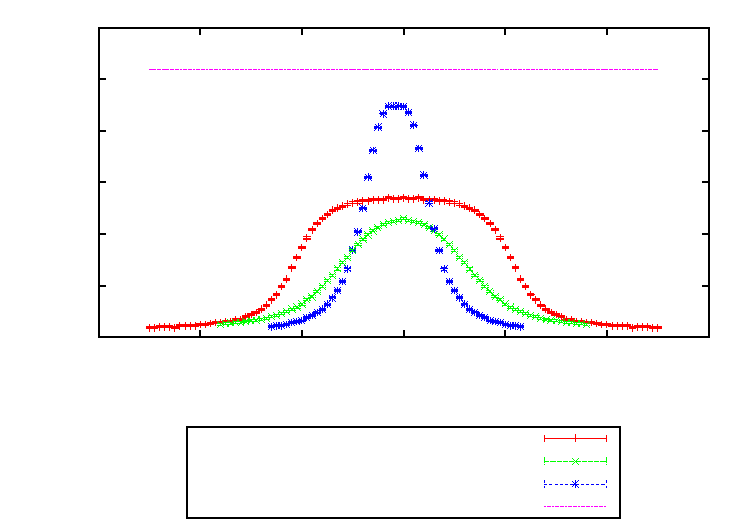
\includegraphics{Homogen}}%
    \gplfronttext
  \end{picture}%
\endgroup

	\caption{Verlauf des Magnetfeldes der 3 Spulen: Messung mit der Hallsonde.}
	\label{fig:Homogen}
\end{figure}

\subsection{Bestimmung von $\mu_0$}
\begin{table}[!htb]
	\centering
	\begin{tabular}{|c|c|c|}
	\hline
	Messungmethode & Spule & $\mu_0$ [$10^{-7}\,\si{\henry\per\meter}$]\\
	\hline
	\hline
	Induktionsspule & Lange Spule & $13.020 \pm 0.020$\\
	\hline
	          & Lange Spule & $13.67 \pm 0.11$ \\
	Hallsonde & Dicke Spule & $13.28 \pm 0.13$ \\
	          & Helmholtzspule & $12.39 \pm 0.05$ \\
	\hline	
	\end{tabular}
	\caption{Aus den verschiedenen Messungen bestimmte Magnetische Feldkonstante}
\end{table}


\section{Diskussion}
\label{sec:diskussion}

\bibliography{literatur}
\bibliographystyle{babalpha}
\end{document}
